\section{Subroutines and Stack}

\subsubsection{Subroutine}

\begin{concept}{Subroutines}
Key elements of subroutines:
\begin{itemize}
  \item Label to identify subroutine entry point
  \item Return instruction (BX LR) to exit
  \item Proper register management
\end{itemize}
\end{concept}





\begin{concept}{Call and Return Mechanism}
Basic subroutine mechanics:
\begin{itemize}
  \item \textbf{BL (Branch with Link)}:
    \begin{itemize}
      \item Stores current PC in LR (R14)
      \item Branches to subroutine address
      \item Direct and relative addressing
    \end{itemize}
  \item \textbf{BLX (Branch with Link and Exchange)}:
    \begin{itemize}
      \item Similar to BL but with register-specified target
      \item Indirect and absolute addressing
    \end{itemize}
  \item \textbf{Return}: Using BX LR or POP {..., PC} if LR was saved
\end{itemize}
\end{concept}

\begin{theorem}{Subroutine Calling Convention and Register Usage}
\begin{itemize}
  \item \textbf{Calling Convention}:
    \begin{itemize}
      \item Parameters passed in R0-R3
      \item Return value in R0
      \item Link Register (LR) for return address
      \item Stack for additional parameters/locals
    \end{itemize}
  \item \textbf{Register Usage}:
    \begin{itemize}
      \item R0-R3: Parameters and scratch
      \item R4-R11: Must be preserved
      \item R12: IP (scratch)
      \item R13: SP (stack pointer)
      \item R14: LR (link register)
      \item R15: PC (program counter)
    \end{itemize}
\end{itemize}
\end{theorem}

\begin{example2}{Subroutine Call and Return}
Multiply by 3 implementation:
\begin{lstlisting}[language=armasm, style=basesmol]
MulBy3  MOV     R4, R0      ; Save input value
        LSLS    R0, #1      ; Multiply by 2
        ADD     R0, R4      ; Add original value
        BX      LR          ; Return
\end{lstlisting}

\begin{minipage}{0.58\linewidth}
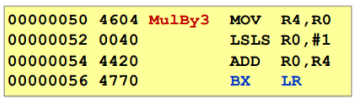
\includegraphics[width=\linewidth]{images/subroutine.png}
\end{minipage}
\begin{minipage}{0.4\linewidth}
in detail:
\begin{itemize}
  \item Label with name \textcolor{darkred}{\textbf{MulBy3}}
  \item Return Statement \textcolor{darkblue}{\textbf{BX LR}}
\end{itemize}
\end{minipage}
\end{example2}

\begin{KR}{Using Subroutines and Stack}
Steps for implementing subroutines:
\begin{enumerate}
  \item Define subroutine entry point with label
  \item Save registers that will be modified
    \begin{itemize}
      \item Use PUSH at start
      \item Include LR if calling other subroutines
    \end{itemize}
  \item Implement subroutine logic
  \item Restore registers in reverse order
    \begin{itemize}
      \item Use POP before return
      \item Can return using POP {..., PC} if LR was saved
    \end{itemize}
  \item Return using BX LR if LR wasn't saved
\end{enumerate}
\end{KR}

\begin{remark}
Important considerations:
\begin{itemize}
  \item Always maintain stack alignment
  \item Match PUSH/POP pairs exactly
  \item Be careful with SP manipulation
  \item Consider nesting depth for stack space
\end{itemize}
\end{remark}

\begin{KR}{Subroutine Implementation}\\
Guidelines for implementing subroutines:

1. Basic subroutine:
\begin{lstlisting}[language=armasm, style=basesmol]
proc_name
    PUSH    {LR}           ; Save return address
    ; Subroutine code
    POP     {PC}           ; Return
\end{lstlisting}

2. With register preservation:
\begin{lstlisting}[language=armasm, style=basesmol]
proc_name
    PUSH    {R4-R7, LR}    ; Save modified registers
    ; Subroutine code using R4-R7
    POP     {R4-R7, PC}    ; Restore and return
\end{lstlisting}

3. With local variables:
\begin{lstlisting}[language=armasm, style=basesmol]
proc_name
    PUSH    {R4, LR}       ; Save registers
    SUB     SP, SP, #8     ; Allocate locals
    ; Use [SP] to [SP, #4] for locals
    ADD     SP, SP, #8     ; Deallocate locals
    POP     {R4, PC}       ; Restore and return
\end{lstlisting}
\end{KR}

\begin{example2}{Nested Subroutine Calls}\\
Example of multiple nested calls with stack manipulation:
\begin{lstlisting}[language=armasm, style=basesmol]
    AREA    progCode, CODE, READONLY
    THUMB
main
    LDR     R1, =0x10203040     ; Initial values
    LDR     R2, =0x50607080
    BL      procA               ; Call procA
    BL      procB               ; Call procB
    B       endless

procA
    PUSH    {R1, R2}            ; Save registers
    LDR     R1, =0xAABBCCDD     ; New values
    LDR     R2, =0xEEFF1020
    POP     {R1, R2}            ; Restore registers
    BX      LR                  ; Return

procB
    PUSH    {R1, R2, LR}        ; Save including LR
    LDR     R1, =0x11223344     ; New values
    LDR     R2, =0x55667788
    BL      procC               ; Call procC
    POP     {R1, R2, PC}        ; Return by popping PC

procC
    PUSH    {R1, R2, LR}        ; Save registers
    LDR     R1, =0x11111111     ; New values
    LDR     R2, =0x22222222
    BL      procD               ; Call procD
    POP     {R1, R2, PC}        ; Return by popping PC
\end{lstlisting}

Stack contents at key points:
\begin{itemize}
  \item After procA PUSH: R1(0x10203040), R2(0x50607080)
  \item After procB PUSH: R1, R2, LR(ret\_addr)
  \item After procC PUSH: R1(0x11223344), R2(0x55667788), LR(ret\_addr)
\end{itemize}
\end{example2}



\subsubsection{Stack}

\begin{definition}{Stack}characteristics:
\begin{itemize}
  \item \textcolor{darkblue}{\textbf{Stack Area}} (Section): Continuous RAM section
  \item \textcolor{darkred}{\textbf{Stack Pointer (SP)}}: R13, points to last written value
  \item \textbf{Direction}: Full-descending (grows toward lower addresses)
  \item \textbf{Alignment}: Word-aligned (4 bytes)
  \item \textbf{Data Size}: 32-bit words only
\end{itemize}

Main operations:
\begin{itemize}
  \item \textcolor{darkgreen}{\textbf{PUSH}}: Decrements SP, then stores words
  \item \textcolor{darkgreen}{\textbf{POP}}: Loads words, then increments SP
\end{itemize}

Stack constraints:
\begin{itemize}
  \item Number of PUSH and POP operations must match
  \item SP must stay between stack-limit and stack-base\\
  $\rightarrow$ \textcolor{darkgreen}{Stack-limit} $\leq$ SP $\leq$ \textcolor{darkpurple}{Stack-base}
\end{itemize}

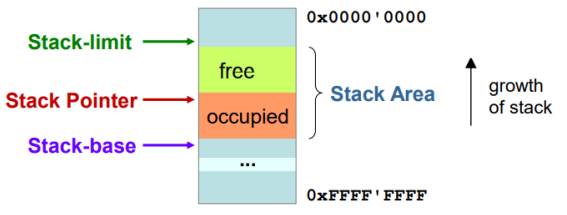
\includegraphics[width=\linewidth]{images/stack_overview.png}


\end{definition}

\begin{concept}{Stack Instructions}
Special stack manipulation instructions:
\vspace{1mm}\\
\begin{minipage}[t]{0.5\linewidth}
\begin{itemize}
  \item \textbf{ADD/SUB SP}:
    \begin{itemize}
      \item Immediate offset 0-508
      \item Must be multiple of 4
    \end{itemize}
  \item \textbf{SP-relative LDR/STR}:
    \begin{itemize}
      \item Immediate offset 0-1020
      \item Used for frame access
    \end{itemize}
\end{itemize}
\end{minipage}
\begin{minipage}[t]{0.5\linewidth}
\begin{itemize}
  \item \textbf{PUSH/POP}:
    \begin{itemize}
      \item Multiple register transfer
      \item Maintains alignment
      \item Can include PC/LR
    \end{itemize}
\end{itemize}
\end{minipage}
\end{concept}



\begin{example2}{PUSH/POP Implementation}

  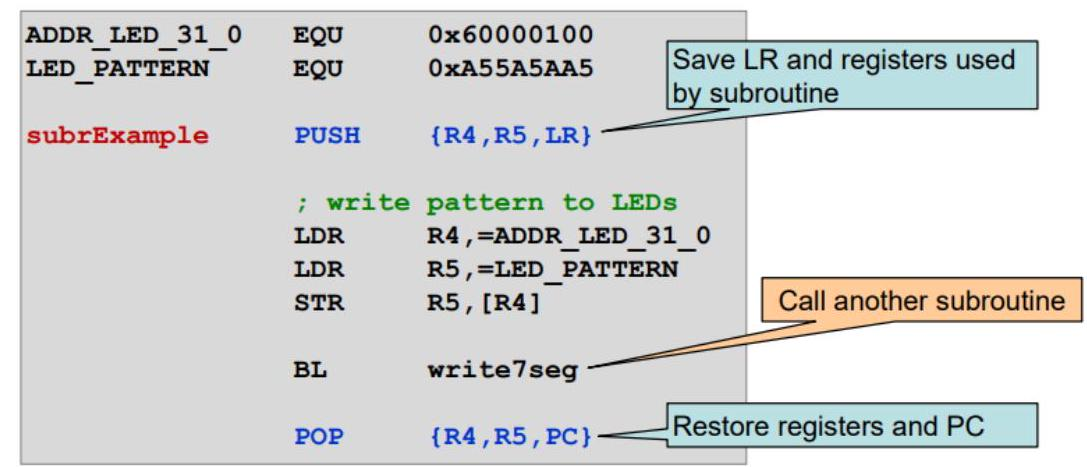
\includegraphics[width=\linewidth]{images/2024_12_29_79e6b22f503fb7b4f718g-08}
\begin{lstlisting}[language=armasm, style=basesmol]
; PUSH {R2,R3,R6}
SUB     SP, SP, #12     ; Reserve stack space
STR     R2, [SP]        ; Store R2
STR     R3, [SP, #4]    ; Store R3
STR     R6, [SP, #8]    ; Store R6

; POP {R2,R3,R6}
LDR     R2, [SP]        ; Restore R2
LDR     R3, [SP, #4]    ; Restore R3
LDR     R6, [SP, #8]    ; Restore R6
ADD     SP, SP, #12     ; Free stack space
\end{lstlisting}
\end{example2}

\subsubsection{Stack Operations and Functions}

\begin{concept}{Stack Operations}
Common stack manipulation patterns:
\begin{itemize}
  \item \textbf{Register Save/Restore}:
    \begin{itemize}
      \item PUSH/POP for callee-saved registers
      \item Multiple register transfer
    \end{itemize}
  \item \textbf{Local Variables}:
    \begin{itemize}
      \item SUB SP to allocate space
      \item Access via SP-relative addressing
      \item ADD SP to deallocate space
    \end{itemize}
  \item \textbf{Return Handling}:
    \begin{itemize}
      \item Save LR if making calls
      \item Return via BX LR or POP \{PC\}
      \item Use PC in POP list when LR saved
    \end{itemize}
\end{itemize}
\end{concept}

\begin{KR}{Function Implementation Patterns}

1. Simple function:
\begin{lstlisting}[language=armasm, style=basesmol]
func    PUSH    {LR}        ; Save return address
        ; Function body
        POP     {PC}        ; Return
\end{lstlisting}

2. Function with locals:
\begin{lstlisting}[language=armasm, style=basesmol]
func    PUSH    {R4, LR}    ; Save registers
        SUB     SP, #8      ; Space for locals
        ; Function body
        ADD     SP, #8      ; Remove locals
        POP     {R4, PC}    ; Return
\end{lstlisting}

3. Function with parameters:
\begin{lstlisting}[language=armasm, style=basesmol]
        ; R0-R3 = first 4 parameters
        ; [SP] = fifth parameter
func    PUSH    {R4-R6, LR} ; Save registers
        LDR     R4, [SP, #16] ; Load 5th param
        ; Function body
        POP     {R4-R6, PC} ; Return
\end{lstlisting}
\end{KR}

\begin{example2}{Stack Frame}
Example of complete function:
\begin{lstlisting}[language=armasm, style=basesmol]
; int calc(int a, int b, int c)
; a in R0, b in R1, c in R2
calc    PUSH    {R4-R6, LR} ; Save registers
        ; Save parameters
        MOVS    R4, R0      ; Save a
        MOVS    R5, R1      ; Save b
        MOVS    R6, R2      ; Save c
        ; Call helper function
        MOVS    R0, R4      ; First param
        BL      helper      ; Call helper
        ; Continue calculation
        ADDS    R0, R5      ; Add b
        ADDS    R0, R6      ; Add c
        
        POP     {R4-R6, PC} ; Return
\end{lstlisting}
\end{example2}

\begin{remark}
Stack usage considerations:
\begin{itemize}
  \item Monitor stack depth in nested calls
  \item Always maintain 8-byte alignment for SP
  \item Consider register usage to minimize stack operations
  \item Be aware of stack space in interrupt handlers
  \item Document stack requirements for functions
\end{itemize}
\end{remark}

\columnbreak

\subsubsection{Stack Frame}

\begin{definition}{Stack Frame Structure}
Components of a stack frame:
\begin{itemize}
  \item \textbf{Saved Registers}:
    \begin{itemize}
      \item Caller-saved (R0-R3, R12)
      \item Callee-saved (R4-R11)
      \item Link register (LR)
    \end{itemize}
  \item \textbf{Local Variables}:
    \begin{itemize}
      \item Allocated on stack if needed
      \item Word-aligned access
    \end{itemize}
  \item \textbf{Parameters}:
    \begin{itemize}
      \item Beyond R0-R3 if needed
      \item Pushed by caller
    \end{itemize}
\end{itemize}

\end{definition}


\begin{KR}{Stack Frame Layout/Management}\\
Steps for function prologue and epilogue, and guidelines for managing stack frames:

1. Frame structure:
\begin{itemize}
  \item Previous stack frame
  \item Return address (LR)
  \item Saved registers
  \item Local variables
  \item Parameters for called functions
\end{itemize}

2. Frame creation/Function prologue:
\begin{lstlisting}[language=armasm, style=basesmol]
    ; Save registers and create frame
    PUSH    {R4-R7, LR}    ; Save registers
    SUB     SP, SP, #frame_size  ; Allocate space
    SUB     SP, SP, #locals ; Allocate local vars
    
    ; Initialize frame if needed
    MOV     R4, #0         ; Clear locals
    STR     R4, [SP, #0]   ; Initialize var1
    STR     R4, [SP, #4]   ; Initialize var2
\end{lstlisting}

3. Stack frame access:
\begin{lstlisting}[language=armasm, style=basesmol]
    ; Access local variables
    LDR     R0, [SP, #offset1]  ; Load local1
    STR     R1, [SP, #offset2]  ; Store to local2

    ; Access parameters
    LDR     R0, [SP, #20]   ; First stack parameter
    ; Access parameters beyond R0-R3
    LDR     R0, [SP, #param_offset] ; Load param
\end{lstlisting}

4. Frame cleanup/Function epilogue:
\begin{lstlisting}[language=armasm, style=basesmol]
    ; Deallocate frame and restore
    ADD     SP, SP, #frame_size  ; Remove locals
    ADD     SP, SP, #locals ; Deallocate locals
    POP     {R4-R7, PC}    ; Restore and return
\end{lstlisting}
\end{KR}

\begin{remark}
Important considerations:
\begin{itemize}
  \item Maintain 8-byte stack alignment
  \item Save LR before any BL instructions
  \item Properly pair PUSH/POP operations
  \item Document stack frame layout
  \item Track stack depth in nested calls
\end{itemize}
\end{remark}



\begin{example2}{Stack Frame Management} Stack frame creation and cleanup:
\begin{lstlisting}[language=armasm, style=basesmol]
func    ; Function prologue
    PUSH    {R4-R8, LR}    ; Save registers
    SUB     SP, SP, #12    ; Allocate locals
    ; Access local variables relative to SP
    STR     R0, [SP, #0]   ; Local var 1
    STR     R1, [SP, #4]   ; Local var 2
    STR     R2, [SP, #8]   ; Local var 3
    ; Function body
    BL      other_func     ; Call another function
    ; Function epilogue
    ADD     SP, SP, #12    ; Deallocate locals
    POP     {R4-R8, PC}    ; Restore and return
\end{lstlisting}
\end{example2}


















